%\vspace{-2mm}
\label{sec:experimental_setup}
To validate the algorithm a load connected to the distribution system containing PV and energy storage was simulated. Figure \ref{fig:system_arch}

\begin{figure}[!htbp]
\centering
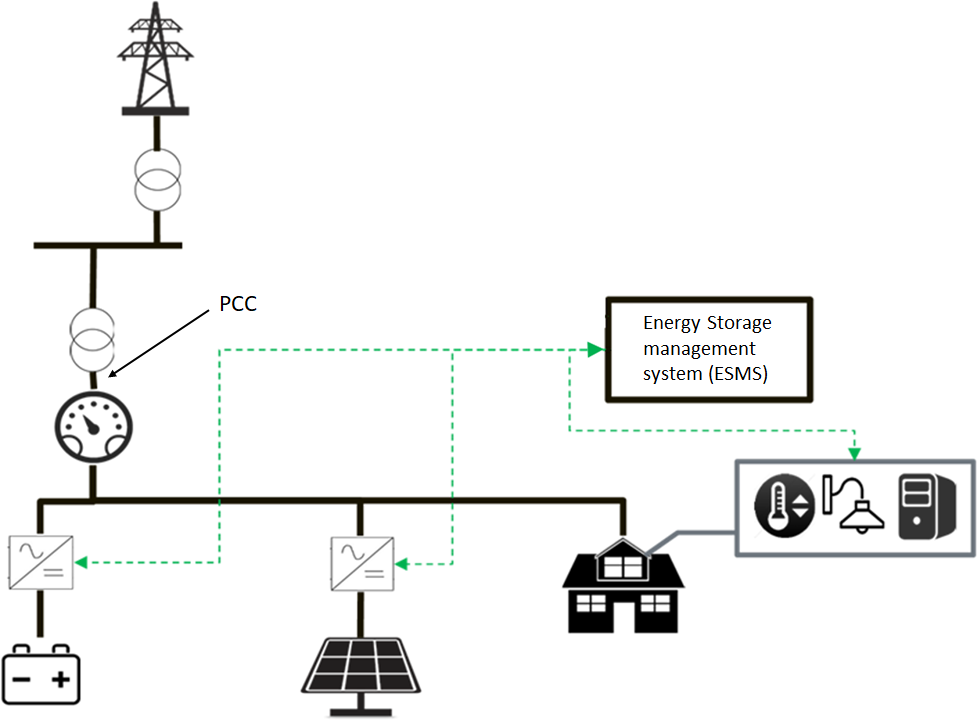
\includegraphics[width=0.45\textwidth]{figs/System_architecture.png}
\caption{Test system architecture}
\label{fig:system_arch}
\vspace{-3mm}
\end{figure}

As seen in the figure the system referenced is a full compared system

For the PV system and the energy storage system, constraints enforced were derived from the physical parameters of the hardware in consideration. The physical bounds (constraints) and price rates associated with the solar power systems are summarized in the Table \ref{tab:solar_pv} and the physical constraints are given by
\vspace{-2mm}
\begin{eqnarray}
\underbar{$Q$}_{_{PV}}\leq Q_{_{PV}}(t_{_k}) \leq \overbar{Q}_{_{PV}}, \\
P^2_{_{PV}}(t_{_k})+Q^2_{_{PV}}(t_{_k})\leq S^2_{_{PV}},
\end{eqnarray}
where
\begin{eqnarray}
\overbar{Q}_{_{PV}}= P_{_{PV}}\tan(\arccos(pf_{_{PV}})),\\
\underbar{$Q$}_{_{PV}}= -P_{_{PV}}\tan(\arccos(pf_{_{PV}})).
\end{eqnarray}


\begin{table}[h]
\caption{Specifications for solar power system used in the study}
\label{tab:solar_pv}
\vspace{-5mm}
\begin{center}
\begin{tabular}{|l|c|}
\hline
PV system parameters & Value \\
\hline
Panels Rating & 875 (kW) \\
\hline
Inverter Rating ($S_{_{PV}}$) & 900 (kVA)\\
\hline
Power Factor ($\rho{f_{_{PV}}}$) Range & 0.8-1.0\\
\hline
Maximum Reactive Power ($\overbar{Q}_{_{PV}}$) & 540 (kVAR)\\
\hline
Minimum Reactive Power ($\underbar{$Q$}_{_{PV}}$) & -540 (kVAR) \\
\hline
LCOE$^*$ ($r_{_{PV}}$) & 2.51 (\textcent/kWh)) \\
\hline
\end{tabular}
\end{center}
$^{*} \text{LCOE: Levelized cost of energy}$
\vspace{-5mm}
\end{table}

The energy storage system constraints and price rates are summarized in Table \ref{tab:energy_storage} and the constraints are given by 
\vspace{-2mm}
\begin{eqnarray}
\overbar{Q}_{_{ES}}= P_{_{ES}}\tan(\arccos(pf_{_{ES}})),\\
\underbar{$Q$}_{_{ES}} = -P_{_{ES}}\tan(\arccos(pf_{_{ES}})),\\
\underbar{$Q$}_{_{ES}}\leq Q_{_{ES}}(t_{_k}), \leq \bar{Q}_{_{ES}},\\
P^2_{_{ES}}(t_{_k})+Q^2_{_{ES}}(t_{_k})\leq S^2_{_{ES}}.
\end{eqnarray}


\begin{table}[h]
\caption{Specifications for energy storage system used in the study}
\vspace{-5mm}
\label{tab:energy_storage}
\begin{center}
\begin{tabular}{|l|c|}
\hline
ESS parameters & Value \\
\hline
Battery Rating & 750 (kW) \\
\hline
Inverter Rating ($S_{_{ES}}$) & 750 (kVA)\\
\hline
Maximum State-of-Charge ($\bar{SOC}_{ES}$) & 2190 (kWh) \\
\hline
Minimum State-of-Charge ($\underbar{SOC}_{_{ES}}$) & 219 (kWh) \\
\hline
Power Factor ($\rho{f_{_{ES}}}$) Range & 0.8-1.0\\
\hline
Maximum Reactive Power ($\overbar{Q}_{_{ES}}$) & 450 (kVAR)\\
\hline
Minimum Reactive Power ($\underbar{$Q$}_{_{ES}}$) & -450 (kVAR) \\
\hline
LCOE$^\star$ ($r_{_{ES}}$) & 12.3 (\textcent/kWh)) \\
\hline
\end{tabular}
\end{center}
$^\star \text{LCOE: Levelized cost of energy}$
%\vspace{-5mm}
\end{table}

To perform the simulations, data related to the distribution network, solar generation profiles, load profiles, and an example feeder were obtained from the available open source databases. The load profile for the distribution network used in this study was obtained from the SUNGRIN project database, which has network model data and load profiles from various feeders located around the state of Florida \cite{sungrin}. Fig. \ref{fig:load_profile} presents an actual load profile with the maximum, minimum, and average power requirement for a 24 h window of a feeder network used in the study. It is important to note that this study used the actual solar irradiance and load profile values obtained from the SUNGRIN project database as the predicted values.  The results will degrade when perfect knowledge does not exist. 

\begin{figure}[!htbp]
\centering
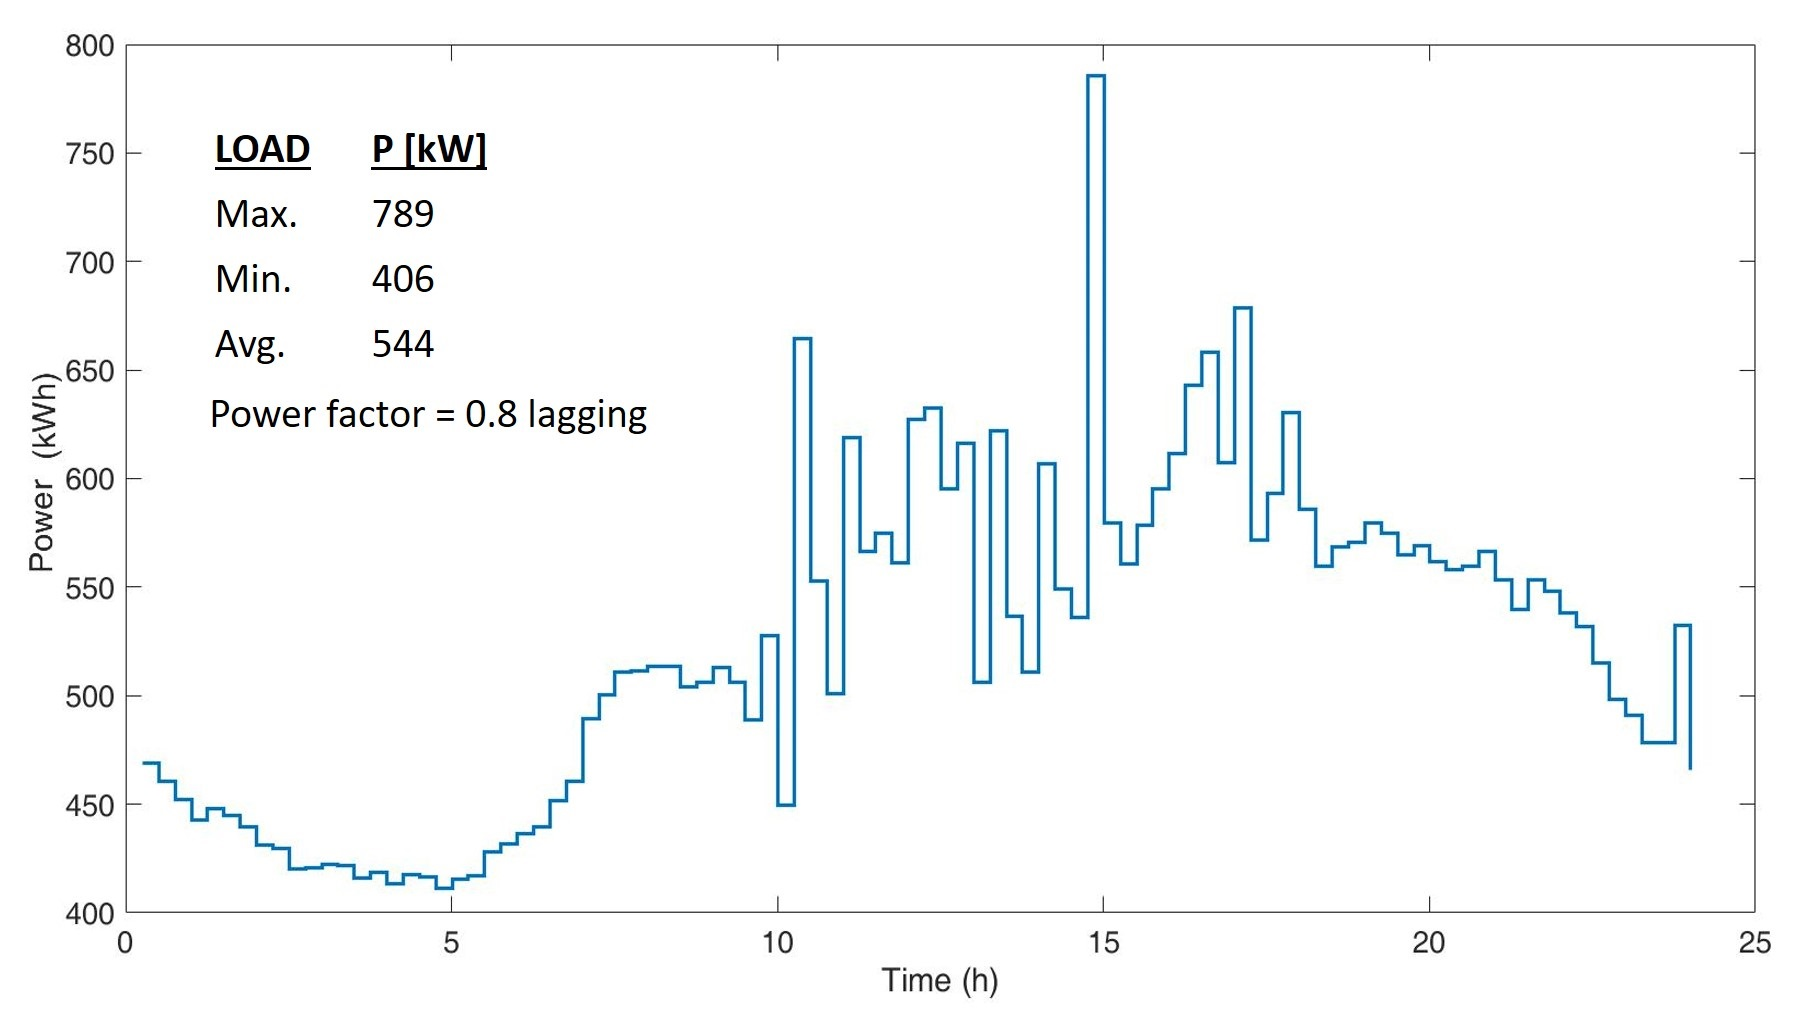
\includegraphics[width=0.45\textwidth]{figs/Load_profile_24hr.jpg}
\caption{Actual load profile with the maximum, minimum, and average power requirement for a 24 h window of a feeder network used in the study.}
\label{fig:load_profile}
\vspace{-3mm}
\end{figure}

As evidenced by the parameters of Tables \ref{tab:solar_pv} and \ref{tab:energy_storage}, the solar power system and ESS were sized for a large-scale (e.g., commercial, industrial or campus scale) micro-grid application. Using the analysis of \cite{res}, $r_{_{ES}}$, the constant levelized cost of energy (LCOE) for the ESS was derived as
\begin{equation}
r_{_{ES}} = \dfrac{ES_{total}}{(Cycles) (ES_{Cap}) (DoD) (\eta_{r})},
\end{equation}
where $ES_{total}$ is the total price of the ESS, $Cycles$ is the total number of cycles under warranty at depth-of-discharge, $ES_{Cap}$ is the total energy capacity of the ESS, $DoD$ is the desired depth-of-discharge of the ESS, and $\eta_{r}$ is the round trip efficiency of the system.


A modified real-time price (RTP) data set was produced using publicly available New York Independent System Operator's (NYISO) wholesale location-based marginal pricing \cite{NYISO2017}. The modification of the price consists of the addition of an RTP supplier charge made by the hypothetical utility company, plus the biasing of an off-peak or on-peak rate determined by using the energy tariff currently available for the TOU program used by the City of Tallahassee. \cite{tallahassee}. The reason for such modification is to preserve the fluctuating nature of the NYISO price data while placing the values in the range of the TOU prices used by the City of Tallahassee, and, therefore more appropriate to North Florida load patterns and markets. The modified RTP values for the 24 h prediction window with a step size of 15 min is shown in Fig. \ref{fig:rtp_24hr}.


\begin{figure}[!htbp]
\vspace{-5mm}
\centering
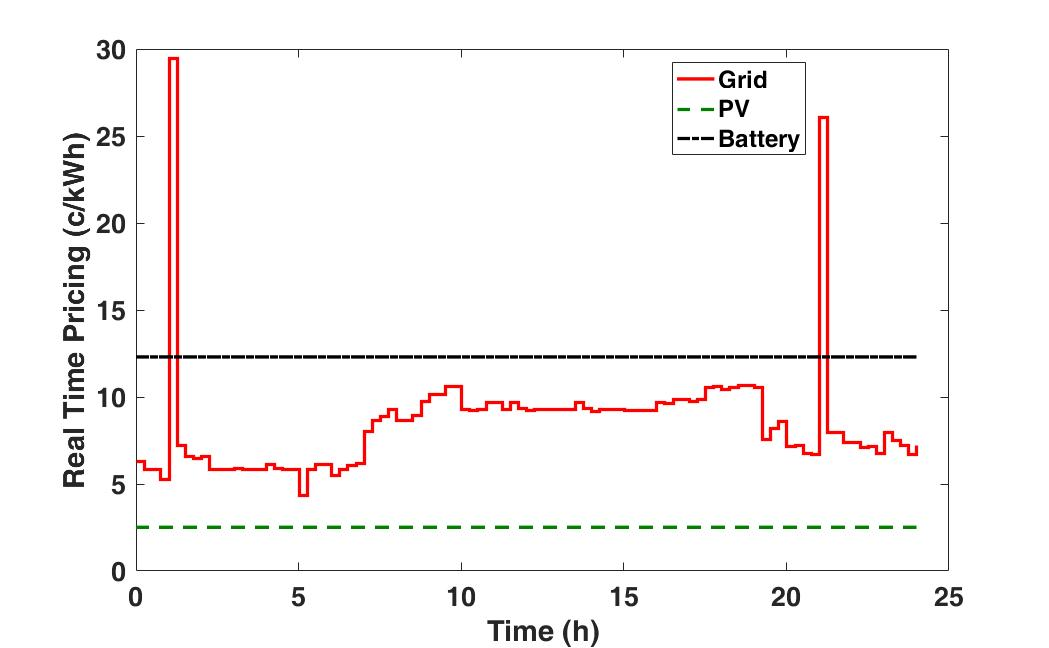
\includegraphics[width=0.5\textwidth]{figs/RTP_24hr_with_der.jpg}
\caption{24 h real-time pricing (RTP) data for grid power for a step size of 15 min used in the study.}
\label{fig:rtp_24hr}
\vspace{-5mm}
\end{figure}

